\documentclass{article}

% Encodings, page setup, paragraph formatting, font
\usepackage[top=0.9in, bottom=1in, left=1.5in, right=1.5in]{geometry}
\usepackage[icelandic]{babel}
\usepackage[T1]{fontenc}
\usepackage[sc]{mathpazo}
\usepackage[parfill]{parskip}
\usepackage{cancel}
\usepackage{comment}
% Tables and lists
\usepackage{booktabs,tabularx}
\usepackage{multirow}
\usepackage{enumerate}
\usepackage{adjustbox}
\usepackage{multicol}
\usepackage{enumitem}
\usepackage{xcolor}
% Math
\usepackage{amsmath, amsfonts, amssymb, amsthm}
\usepackage{gensymb}
% Graphics
\usepackage{graphicx}
\usepackage{forest}
\usepackage{tikz}
\usetikzlibrary{positioning, shapes, arrows.meta}
% Code environment
\usepackage{listingsutf8}
\definecolor{commentcolor}{RGB}{0, 128, 0} % Grænn
\definecolor{keywordcolor}{RGB}{0, 0, 255}   % Blár
\definecolor{stringcolor}{RGB}{163, 21, 21}      % Dökkrauður
\definecolor{numbercolor}{RGB}{128, 0, 128}      % Fjólublár
\definecolor{identifiercolor}{RGB}{0, 0, 0}      % Svartur

\lstset{
    language=Java,
    basicstyle=\ttfamily,
    keywordstyle=\color{keywordcolor}\bfseries,
    commentstyle=\color{commentcolor},
    identifierstyle=\color{identifiercolor},
    stringstyle=\color{stringcolor},   
    showstringspaces=false,
    numbers=left,
    numberstyle=\tiny\color{gray},
    tabsize=2,
    breaklines=true,
    columns=fullflexible,
    keepspaces=true,
    inputencoding=utf8, 
    extendedchars=true,  
    literate=
        {á}{{\'a}}1
        {ð}{{\dh}}1
        {é}{{\'e}}1
        {í}{{\'i}}1
        {ó}{{\'o}}1
        {ú}{{\'u}}1
        {ý}{{\'y}}1
        {þ}{{\th}}1
        {æ}{{\ae}}1
        {ö}{{\"o}}1
        {Á}{{\'A}}1
        {Ð}{{\DH}}1
        {É}{{\'E}}1
        {Í}{{\'I}}1
        {Ó}{{\'O}}1
        {Ú}{{\'U}}1
        {Ý}{{\'Y}}1
        {Þ}{{\TH}}1
        {Æ}{{\AE}}1
        {Ö}{{\"O}}1,
}

% Restin af forskriftinni
\usepackage[pdftex,bookmarks=true,colorlinks=true,pdfauthor={Hafsteinn Einarsson},linkcolor=blue,urlcolor=blue]{hyperref}

% Hyphenation
\hyphenpenalty=5000
% Page and section numbering
\setcounter{secnumdepth}{-1} 
\pagenumbering{gobble}

\title{Tölvugrafík Lokaprófa undirbúningur}
\author{brj46 }
\date{Nóvember 2024}

\begin{document}

\maketitle

\vspace {7em}
\begin{center}

\includegraphics[width=0.7\textwidth]{myndir/3d.jpg}
\end{center}

\newpage
\section*{Hvað Þarf Ég Að Kunna?}

\begin{itemize}
    \item[$\square$] Varpanir (tvívíðar og þrívíðar) (töluleg rök)
    \item[$\square$] Hreyfanleg líkön (WebGl) (Render-Föll)
    \item[$\square$] Endurskinslíkön (Phong lýsingarlíkanið) (útreikningar með dofnun)
    \item[$\square$] Mynsturvörpun (Texture mapping t.d. repeat og \text{CLAMP\_TO\_EDGE}) Ójafnhliða síun
    \item[$\square$] GLSL og litaraforritun (Hnúta- og bútalitarar) (Hreyfing og litabreytingar)
    \item[$\square$] Ýmis atriði í tölvugrafík (Homogeneous hnit) (þríhyrnaröðun)(Skuggakort)
    \item[$\square$] Aukaverkefni (Geislasmölun vs Phong) (Dofnun og birtustýring)
\end{itemize}

\newpage

\section{Mín lausn við prófinu 2023}

\subsection{Varpanir}
\subsubsection{a.} Á myndinni er gefin upphafsstaða á húsi í tvívídd. Neðra vinstra horn þess er i (1, 2).

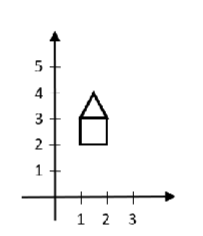
\includegraphics[scale = 0.9]{myndir/mynd2023a.png}

Teiknið mynd af stöðu hússins eftir þessar samsettu varpanir (hvor liður sjálfstæður). Rökstyðjið í nokkrum orðum hver útkoman er.

\begin{itemize}
    \item[i.] $T(1, 2)*S(1, 2)*T(2,-1)*R(90\degree)$

    \item \textbf{Svar mitt} Alright skoðum hverja skipun fyrir sig (lesum frá hægri til vinstri) R($90\degree$) mun snúa húsinu um 90 gráður en frá 0.0 og snúið til vinstri svo næsta staða hússins væri
    \item[2. $R(90\degree)$] 
    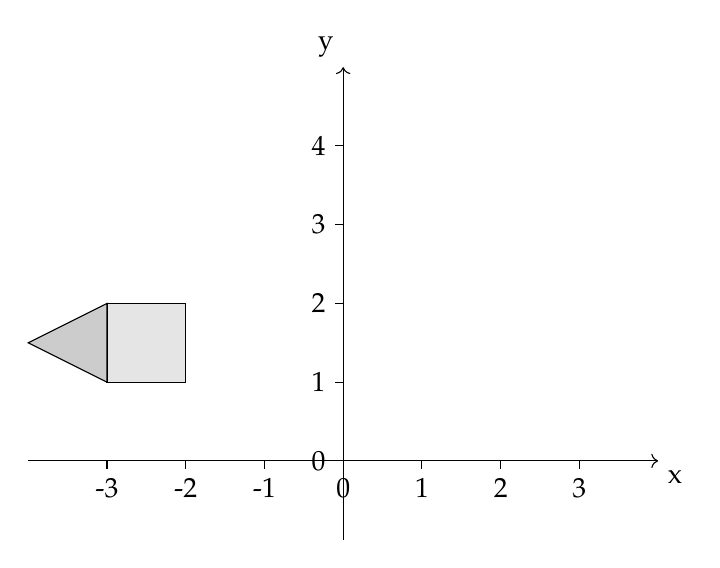
\begin{tikzpicture}
        \draw[->] (-4,0) -- (4,0) node[anchor=north west] {x};
        \foreach \x in {-3, -2, -1, 0, 1, 2, 3}
        \draw (\x, 0) -- (\x, -0.1) node[anchor=north] {\x};
        
        \draw[->] (0,-1) -- (0,5) node[anchor=south east] {y};
        \foreach \y in {0, 1, 2, 3, 4} 
        \draw (0, \y) -- (-0.1, \y) node[anchor=east] {\y};
        
        \draw[fill=gray!20] (-3, 1) rectangle (-2, 2);

        \draw[fill=gray!40] (-3, 1) -- (-4, 1.5) -- (-3, 2) -- cycle; 
        
    \end{tikzpicture}

    Næst er T(2,-1) þá munum við færa húsið 2 til hægri og 1 niður.

    Svo er skölunin S(1, 2) sem mun skala húsið með 1 í x-ás og 2 í y-ás. semsagt tvöfaldast upp og viðheldur breiddinni.

    Síðast er T(1, 2) sem færir húsið 1 til hægri og 2 upp.

    að lokum höfum við
    
    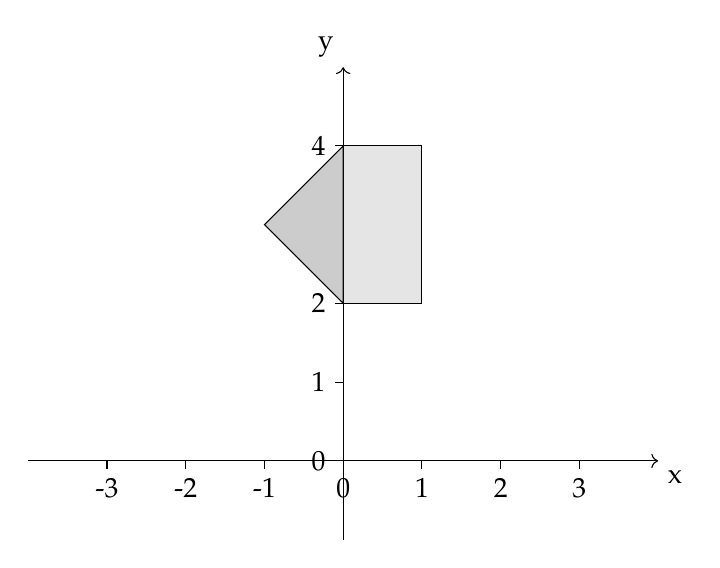
\begin{tikzpicture}
        \draw[->] (-4,0) -- (4,0) node[anchor=north west] {x};
        \foreach \x in {-3, -2, -1, 0, 1, 2, 3}
        \draw (\x, 0) -- (\x, -0.1) node[anchor=north] {\x};
        
        \draw[->] (0,-1) -- (0,5) node[anchor=south east] {y};
        \foreach \y in {0, 1, 2, 3, 4} 
        \draw (0, \y) -- (-0.1, \y) node[anchor=east] {\y};
        
        \draw[fill=gray!20] (0, 2) rectangle (1, 4);

        \draw[fill=gray!40] (0, 2) -- (-1, 3) -- (0, 4) -- cycle; 
        
    \end{tikzpicture}








    \item[ii.] $T(1, 2)*R(90\degree)*S(1,2)*T(-1,-2)$

    \item \textbf{Svar mitt} Jæja taka tvö ég hafði gert fyrra dæmið í heimdæmi svo ég var svoldið með það skulum gera þetta núna 

    Sama dæmi byrjum á að lesa frá hægri til vinstri. 
    
    T(-1, -2) færir húsið 1 til vinstri og 2 niður.

    S(1, 2) skalar húsið með 1 í x-ás og 2 í y-ás.

    R($90\degree$) snýr húsinu um 90 gráður til vinstri muna það því mér þykir það weird að snúa húsinu til vinstri.

    Síðast er T(1, 2) færir húsið 1 til hægri og 2 upp.

    að lokum höfum við

    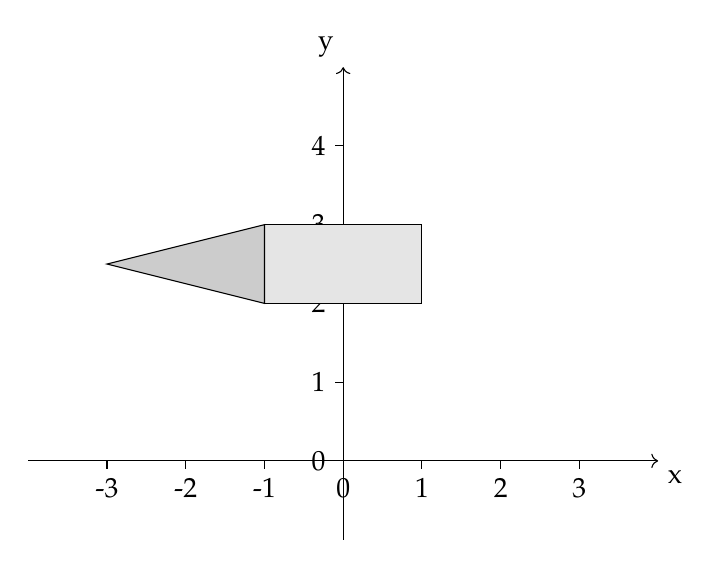
\begin{tikzpicture}
        \draw[->] (-4,0) -- (4,0) node[anchor=north west] {x};
        \foreach \x in {-3, -2, -1, 0, 1, 2, 3}
        \draw (\x, 0) -- (\x, -0.1) node[anchor=north] {\x};
        
        \draw[->] (0,-1) -- (0,5) node[anchor=south east] {y};
        \foreach \y in {0, 1, 2, 3, 4} 
        \draw (0, \y) -- (-0.1, \y) node[anchor=east] {\y};
        
        \draw[fill=gray!20] (1, 2) rectangle (-1, 3);

        \draw[fill=gray!40] (-1,2) -- (-3, 2.5) -- (-1, 3) -- cycle; 
        
    \end{tikzpicture}
\end{itemize}

\newpage

\subsubsection{b.} Sýnið samsetta tvívíða vörpun sem breytir ferningnum í fyrri myndinni yfir í
ferhyrninginn í seinni myndinni. Seinni ferhyrningurinn er með miðpunkt (2,
2), hliðarlengdir 1 og 2, og halli hans er $45\degree$. Rökstyðjið einstakar
grunnvarpanir í samsettu vörpuninni.

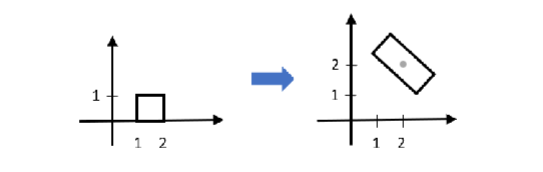
\includegraphics[scale = 0.9]{myndir/mynd2023b.png}

\newpage

\subsection{2} WebGl Útfærsla á líkani

Það er til útgáfa af klukku (Continue Time, hönnuður Sander Mulder) sem hefur
þrjá arma eins og venjuleg klukka, en í stað þess að armarnir
snúist allir um sama punkt (þ.e. miðpunkt skífu), þá eru þeir
festir á endann á öðrum armi. Klukkustundararmurinn er
reyndar festur á miðpunkt skífu og snýst um hann eins og á
venjulegri klukku, en mínútuarmurinn er festur á endann á
klukkustundararminum og snýst um þann punkt. Sömuleiðis
er sekúntuarmurinn festur á endann á mínútuarminum og
snýst um hann. Á myndinni hér til hliðar er
klukkustundararmurinn á milli 4 og 5, mínútuarmurinn sýnir
30 og sekúntuarmurinn vísar á 45. Klukkan hér er því
4:30:45.

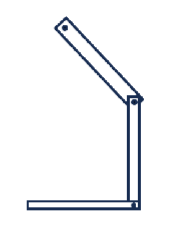
\includegraphics[scale = 0.9]{myndir/klukka.png}

Sýnið uppkast að render-falli sem teiknar þessa klukku. Hver armur á að vera
teningur og þið getið gert ráð fyrir að sé búið að hlaða hnúta hans inn í
grafíkminni. Vísarnir eiga að liggja í xy-sléttunni og þeir eiga að snúast rétt,
þannig að fyrir hvern heilan hring sekúntuarmsins snýst mínútuarmurinn sem
svarar einni mínútu (þ.e. 1/60 af heilum hring). Samsvarandi gildir með
klukkustundararminn. Þið eigið bara að uppfæra sekúntuarminn um eina sekúntu í
hverri ítrun render-fallsins (og hina armana samsvarandi). Þetta gefur auðvitað
ekki réttan tíma, en sýnir hreyfingu klukkunnar.
Einbeitið ykkur að því að sýna varpanirnar og teikniföllin í render-fallinu. Þetta
þarf ekki að vera alveg keyranlegur kóði, heldur skiptir meira máli að þið séuð að
hugsa varpanirnar rétt. Útskýrið þess vegna vel einstakar skipanir.


\textbf{Svar}:
\begin{lstlisting}
function render()
{
    gl.clear( gl.COLOR_BUFFER_BIT | gl.DEPTH_BUFFER_BIT);

    var proj = perspective( 70.0, 1.0, 0.2, 10.0 );
    gl.uniformMatrix4fv(proLoc, false, flatten(proj));
    
    var mv = lookAt( vec3(0.0, 0.0, zDist), vec3(0.0, 0.0, 0.0), vec3(0.0, 1.0, 0.0) );
    mv = mult( mv, rotateX( spinX ) );
    mv = mult( mv, rotateY( spinY ) );
    
    // Ba til bakgrunn fyrir klukku
    mvb = mult( mv, translate( 0.0, 0.0, -0.04 ) );
    mvb = mult( mvb, rotateY( 180.0 ) );
    mvb = mult( mvb, scalem( 1.25, 1.25, 0.01 ) );
    gl.uniformMatrix4fv(mvLoc, false, flatten(mvb));
    gl.drawArrays( gl.TRIANGLES, 0, NumVertices );
    


    sek += sekupph;
    sekvisir = 6*sek;
    minvisir = 0.1*sek;
    kstvisir = 0.1*sek/11.0;


    // ---------- Klukkustundavísir
    mv = mult( mv, rotateZ( -kstvisir ) );              // Sna samkvmt breytingu  tma
    
     // Líkanavörpun klukkustundavisis
    mvk = mult( mv, translate( 0.0, 0.1, 0.0 ) );       // Hlira upp, svo neri endi  (0, 0, 0)
    mvk = mult( mvk, scalem( 0.025, 0.2, 0.025 ) );       // Setja  rtta str

    gl.uniformMatrix4fv(mvLoc, false, flatten(mvk));
    gl.drawArrays( gl.TRIANGLES, 0, NumVertices );


    // ---------- Mínútuvísir
    mv = mult( mv, translate( 0.0, 0.2, 0.0 ) );        // Fra t  enda klukkustundavsis
    mv = mult( mv, rotateZ( -minvisir ) );              // Sna samkvmt breytingu  tma
    
     // Lkanavrpun mntuvsis
    mvm = mult( mv, translate( 0.0, 0.1, 0.0 ) );       // Hlira upp, svo neri endi  (0, 0, 0)
    mvm = mult( mvm, scalem( 0.02, 0.2, 0.02 ) );       // Setja  rtta str

    gl.uniformMatrix4fv(mvLoc, false, flatten(mvm));
    gl.drawArrays( gl.TRIANGLES, 0, NumVertices );

    
    // ----------- Seknduvsir
    mv = mult( mv, translate( 0.0, 0.2, 0.0 ) );        // Fra t  enda mntuvsis
    mv = mult( mv, rotateZ( -sekvisir ) );              // Sna samkvmt breytingu  tma
    
     // Lkanavrpun seknduvsis
    mvs = mult( mv, translate( 0.0, 0.1, 0.0 ) );       // Hlira upp, svo neri endi  (0, 0, 0)
    mvs = mult( mvs, scalem( 0.015, 0.2, 0.015 ) );       // Setja  rtta str

    gl.uniformMatrix4fv(mvLoc, false, flatten(mvs));
    gl.drawArrays( gl.TRIANGLES, 0, NumVertices );


    requestAnimFrame(render);
}

\end{lstlisting}

\newpage

\subsection{3.} Endurskinslíkön

Hér fyrir neðan er líkan með áhorfanda, ljósgjafa og glansandi yfirborði.
Áhorfandinn og ljósgjafinn eru í sömu hæð og beint fyrir ofan sitthvort brotið í
yfirborðinu. Gerið ráð fyrir að notað sé endurskinslíkan Phong án dofnunar til að
búa til lit á yfirborðið.

\begin{center}
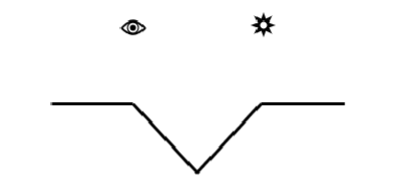
\includegraphics[scale = 0.9]{myndir/Endurskin.png}
\end{center}


\subsubsection{a.}Hvar á yfirborðinu er bjartasta \underline{dreif}endurskin (diffuse reflection)? Ef fleiri en
einn staður eru jafnbjartir tilgreinið þá alla björtustu staðina. Rökstyðjið
svarið í nokkrum orðum.

\subsubsection{b.}Hvar á yfirborðinu er bjartasta \underline{depil}endurskin (specular reflection)? Ef fleiri
en einn staður eru jafnbjartir tilgreinið þá alla björtustu staðina. Rökstyðjið
svarið í nokkrum orðum.

\subsubsection{c.}Ef hægt væri að færa ljósið til hliðar (í sömu hæð), eru staðsetningar á ljósinu
sem gefa ekkert depilendurskin á þessu yfirborði? Gerið ráð fyrir að
glansstuðull yfirborðsins sér hár og depillinn sé því lítill. Rökstyðjið svarið.

\subsubsection{d.}Ef ekkert \underline{umhverfis}endurskin (ambient reflection) væri í líkaninu, væri þá
einhver hluti yfirborðsins alveg svartur? Rökstyðjið.

\newpage

\subsection{4.} Ýmislegt efni

Hér fyrir neðan eru stuttar spurningar úr ýmsu efni námskeiðsins. Svarið hverri
spurningu með nokkrum setningum

\subsubsection{a.}Berið saman Gouraud litun og Phong litun. Nefnið einn kost og einn galla
við hvora aðferð.

\subsubsection{b.}Er hægt að útfæra mynsturvörpun eingöngu í hnútalitara? Rökstyðjið svar
ykkar.

\subsubsection{c.}Skuggakort (shadow maps) eru ein leið til að fá skugga í WebGL. Lýsið
stuttlega hvernig hún virkar og hvaða takmarkanir eru á aðferðinni.

\subsubsection{d.}Útskýrið hvaða kosti það hefur að nota jafnþætt (homogeneous) hnit í
tölvugrafík.

\subsubsection{e.}Hvers vegna skiptir máli að röð hnúta í þríhyrningi sé rétt (þ.e. rangsælis eða
réttsælis)? Rökstyðjið.

\newpage

\subsection{5.} Mynsturvörpun

\subsubsection{a.}Spurningar um ójafnhliða síun (anisotropic filtering):

\begin{itemize}
    \item[i.]Hvers vegna er ójafnhliða síun betri en "trilinear" síun (þ.e. MIP vörpun
    með \textbf{LINEAR-LINEAR} stillingu) á gólfi sem teygir sig langt frá áhorfanda?
    Rökstyðjið.
    \item[ii.]Eru einhver tilvik þar sem ójafnhliða síun gæfi verri útkomu en "trilinear"
    síun? Rökstyðjið.
\end{itemize}

\subsubsection{b.}Hér fyrir neðan eru þrjár myndir af spjaldi þar sem búið er að
varpa á það mynstrinu af tepottinum hér til hægri. Í hverju
tilfelli gefið mynsturhnitin sem þarf að nota og tiltakið þær
stillingar á mynsturvörpuninni sem skipta máli til að fá þessa
útkomu.

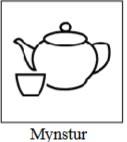
\includegraphics[scale = 0.9]{myndir/mynstur.png}

\begin{center}
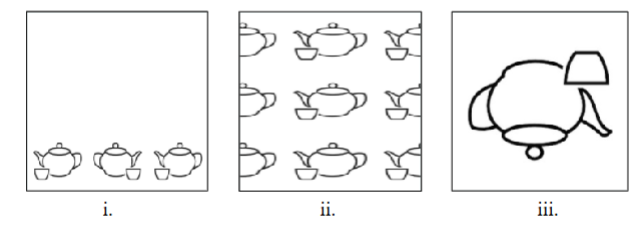
\includegraphics[scale = 0.9]{myndir/mynstur2.png}
\end{center}


\newpage

\subsection{6.} Bakhliðareyðing og litaraforritun

\subsubsection{a.}Segjum að við litum margflötung (polytope) með endurskinslíkani Phong og
Phong litun. Ef það er ljósgjafi fyrir aftan margflötunginn (frá áhorfanda) og
ef bakhliðareyðing (back-face culling) \underline{er ekki virk}, hvernig lit fá þá bakhliðar
margflötungsins (ef við sæjum inn í hann)? Rökstyðjið

\subsubsection{b.}Hvernig breytist svar ykkar í a-lið ef bakhliðareyðing \underline{er virk}? Rökstyðjið.

\subsubsection{c.}GLSL bútalitarar hafa innbyggðu breytuna \text{\textbf{gl\_FrontFacing}}. Þetta er
breyta af taginu \underline{bool} sem er sönn ef núverandi bútur er hluti af þríhyrningi
sem snýr að áhorfandanum, en ósönn annars. Skrifið GLSL kóðabút sem
veldur því að allar bakhliðar sem sjást eru rauðar, en framhliðar væru litaðar
eins og venjulega (þið þurfið ekki að skrifa út þann hluta kóðans!). Hvað
myndi gerst í kóðanum ykkar ef bakhliðareyðing væri virk? Útskýrið.

\end{document}